\chapter{Interviews Documentation \label{cha:interviews}}

This appendix provides the supporting documents used in the study of \LLLs
requirements described in Chapter \ref{cha:model}. The following documents are:

\begin{itemize}
  \item Scenarios used in interviews with lecturers.
  \item Questions used in interviews with lecturers.
  \item Scenarios used in interviews with students.
  \item Questions used in interviews with students.
\end{itemize}

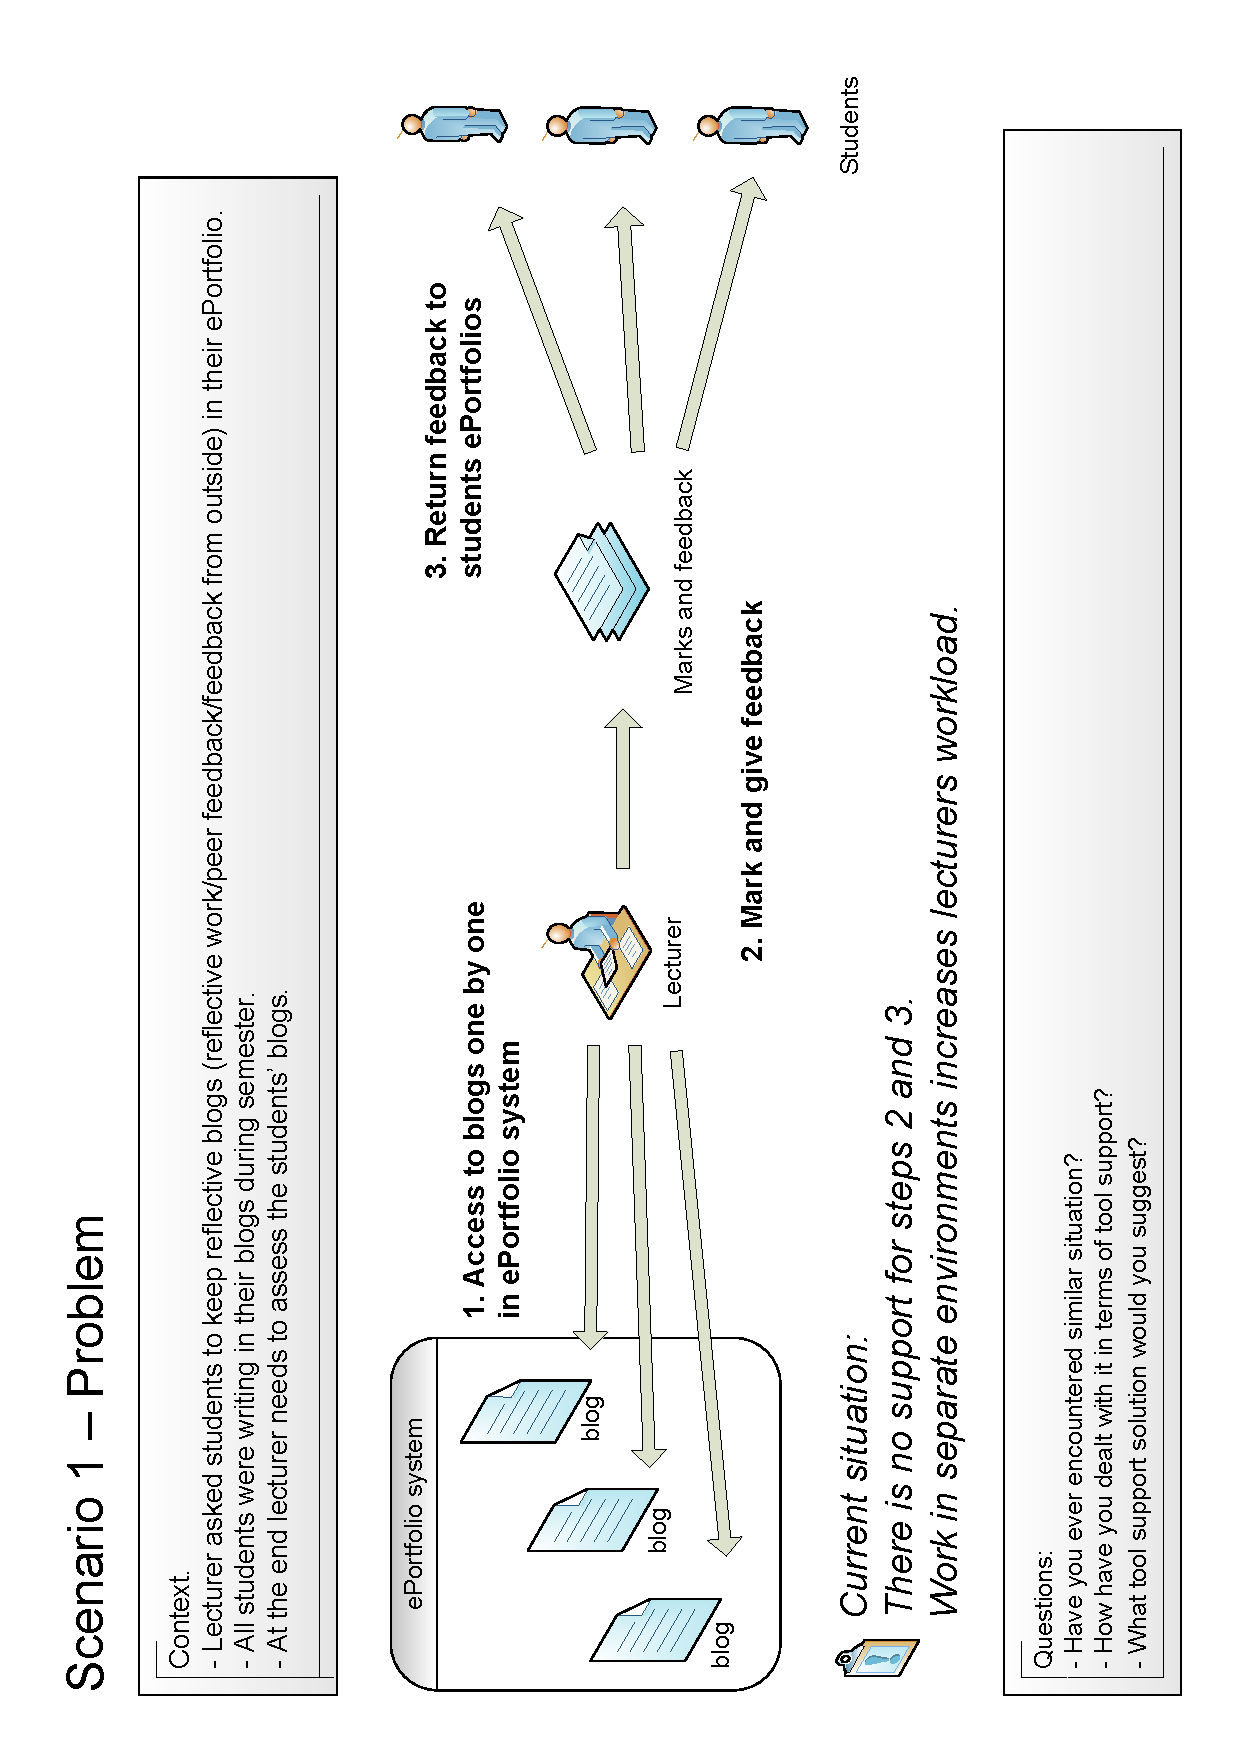
\includepdf[scale=0.7,pages=1,pagecommand=\section{Lecturer Scenario
Examples}\label{sec:appscenariolect},frame]{appendix/Scenarios_L.pdf}

\includepdf[scale=0.75,pages=2,pagecommand={},frame]{appendix/Scenarios_L.pdf}

\includepdf[scale=0.75,pages=3,pagecommand={},frame]{appendix/Scenarios_L.pdf}

\includepdf[scale=0.75,pages=4,pagecommand={},frame]{appendix/Scenarios_L.pdf}

\section{Guiding questions for the interviews with lecturers}
\label{sec:appquestlect}
\begin{itemize}
\item What is your role as a teacher within the \ep~system at the university?

\item What is your experience of using LMS and \ep~systems with students at the
university?

\item What do you see as the biggest problems or inefficiencies with using these
systems?

\item Can you describe some specific areas of strengths and weaknesses of the
\ep~system you have used?

\item What do you think you need to be able to accept an \ep~system? What
would be your conditions for its use by students?

\item Looking at LMS from a different perspective, could you add anything to it
which is outside its core functionality that would support students in \LLLsn?

\item What would you like to do that your \ep~system does not allow you to do
now, so that it could become more useful and relevant to \LLLs support in
universities?

\item What would you expect a system designed for supporting \LLLs provide for
students?

\item What other features would you like to see in environments which support
students in \LLLs in universities?

\item To sum up, we discussed such features as \ldots. Which of them do you
think are the most important for a student-centred \LLLs environment?
\end{itemize}

\includepdf[scale=0.7,pages=1,pagecommand=\section{Student Scenario
Examples}\label{sec:appscenariostud},frame]{appendix/Scenarios_S.pdf}

\includepdf[scale=0.75,pages=2,pagecommand={},frame]{appendix/Scenarios_S.pdf}

\includepdf[scale=0.75,pages=3,pagecommand={},frame]{appendix/Scenarios_S.pdf}

\includepdf[scale=0.75,pages=4,pagecommand={},frame]{appendix/Scenarios_S.pdf}

\includepdf[scale=0.75,pages=5,pagecommand={},frame]{appendix/Scenarios_S.pdf}

\section{Guiding questions for the interviews with students}
\label{sec:appqueststud}
\begin{itemize}
\item What is your experience of using LMS and \ep~systems at the university? 

\item Can you describe some specific areas of strengths and weaknesses of the
\ep~system you have used? 

\item What would you like to do that your \ep~system does not allow you to do
now, so that it could become more useful and relevant to \LLLs support in
universities?

\item What do you see as the biggest problems or inefficiencies with using
\ep~systems?

\item What features would you like to see in environments that could support
your \LLLs at the university?

\item To sum up, we discussed such features as \ldots. Which of them do you
think are the most important for an environment that provides support for your
\LLLsn?
\end{itemize}